%D�finir le format du document: papier, taille de police, type de document, etc.
\documentclass[a4paper, 11pt]{article}

%%%%%%%%% Packages externes utilis�s %%%%%%%%%%%%%%%%%%%
\usepackage[french]{babel}
\usepackage[latin1]{inputenc}
\usepackage[T1]{fontenc}
\usepackage{verbatim}
\usepackage{graphicx}
\usepackage{epstopdf}
\usepackage{macro}
\usepackage{algorithm}
\usepackage{algorithmic}
%\usepackage{algorithm2e}


%La mise en page du rapport, NE PAS MODIFIER.
\usepackage{geometry}
 \geometry{
 a4paper,
 left=20mm,
 right=20mm,
 top=20mm,
 bottom=20mm,
 }

%%%%%%%%% Le corps du document entre begin et end %%%%%%%%%%%%%%%%%%%
\begin{document}

%Page de garde
%%%%%%%%%%%%%%% Page de garde %%%%%%%%%%%%%%%%%%%

\begin{titlepage}{
    \begin{center}
        \vspace* {25mm}
        {\Large \textbf {Universit� de Cergy-Pontoise}} \\
        \vspace* {10mm}
        {\Large \textbf {RAPPORT}} \\
        \vspace* {10mm}
        pour le projet G�nie Logiciel \\
        \textbf {Licence d'Informatique deuxi�me ann�e} \\
        \vspace* {10mm}

	sur le sujet \\
        \vspace* {10mm}
	{\Huge \textsf{Urbain}} \\
        \vspace* {10mm}
 	r�dig� par \\
        \vspace* {10mm}
        {\Large \textbf {Matthieu VILAIN et Quentin GERARD}} \\
				\vspace* {10mm}
				\noreffig{images/ville.png}{12.82cm}{8.2cm} \\
        \date Mai 2015
        \vspace* {10mm}
	\end{center}
}
\end{titlepage}

%G�n�ration automatique de la table des mati�res, de la liste des figures et de la liste des tableaux
\tableofcontents
\listoffigures
\listoftables

%Une section "remerciements" pourrait �tre int�ressante. C'est une section non num�rot� (avec un * )
\section*{Remerciements}
Les auteurs du projet voudraient remercier...

\section{Introduction}
\label{sec:introduction}

\paragraph{Le projet}
Le projet consiste � la cr�ation d'un jeu vid�o simulant une vie urbaine, dans laquelle
plusieurs individus vivent leur vie au sein d'une ville. L'utilisateur pourra infuer sur le comportement
des individus et les param�tres de la ville.

\paragraph{Fonctionnalit�s} Fonctionnalit�s du programme:
Le joueur aura plusieurs actions possibles afn d'infuer sur l'�volution de la ville. Tout
d'abord il pourra agir sur le temps en l?acc�l�rant ou en le mettant en pause. Ensuite il pourra acc�der
� des informations sur les personnages comme : leurs informations de bases, leur historique ou leurs
objectifs directs (exemple : ce personnage se rend � la piscine). Ces informations pourront �tre
chang�es par l'utilisateur et il pourra ainsi renommer un personnage, le faire d�m�nager ou le faire
rentrer chez lui par exemple. De m�me pour les b�timents, l'utilisateur pourra acc�der � ses
informations et les modifer. Il pourra donc par exemple modifer les horaires d'ouverture d'un lieu ou
faire varier son nombre d'utilisateur maximum. Le joueur pourra donc modifer � sa guise ses
informations et voir ce que ces modifcations apportent de bon ou de mauvais sur � population de la
ville.

\paragraph{Nos motivations}
Nous avons choisi ce projet car il repr�sente une opportunit� pour chacun de nous
d?explorer des domaines/notions qui nous int�ressent, et dans lesquelles nous voulons nous
perfectionner.

\section{Sp�cification}
\label{sec:specification}

\paragraph{Chapeau} Nous avons pr�sent� l'objectif du projet dans la section \ref{sec:introduction}. Dans cette section, nous pr�sentons la sp�cification de notre logiciel r�alis�. Ceci correspond principalement au cahier des charges.

\subsection{Premi�re sous-section}
\label{sec:spec1}

\paragraph{Premier paragraphe} On commence � expliquer...

\paragraph{} Juste un simple paragraphe.

\subsection{Deuxi�me sous-section}
\label{sec:spec2}

\begin{table}[h!]
\centering
\begin{tabular} {|p{3.5cm}|p{2.5cm}|p{5cm}|}
\hline
Document & Coefficient & Commentaire \\
\hline
Cahier des charges & 37.5\% & Premier document \\
\hline
Rapport & 62.5\% & Rapport final du projet \\
\hline
\end{tabular}
\caption{Documents � remettre}
\label{tab:document}
\end{table}

Comme ce qui est illustr� dans le tableau \ref{tab:document}, ...

\section{R�alisation}
\label{sec:impl}

%\begin{figure}
%\centering
%
\includegraphics[width=3.5cm, height=2cm]{images/programmer.png}
%\caption{Un programmeur occup�}
%\label{fig:modele}
%\end{figure}

\subsection{Le Model - pr�sentation des classes}

\subsubsection{La ville}

La ville est le premier �l�ment qui constitue notre projet. Elle est compos�e de diff�rentes infrastructures�: Les routes, les maisons, les b�timents de travail et les divertissements. Chaque type d'infrastructure poss�de une utilit� qui lui est propre�:
\begin{itemize}
 \item Les Routes permettent aux personnages de se d�placer
 \item Les Maisons permettent aux personnages de se reposer le soir et regagner de l'�motion
 \item Le Travail est une activit� impos� � chaque personnages et sera la principale source de baisse d'�motion
 \item Les Divertissements permettent aux personnages lorsqu'ils ne dorment pas de regagner de l'�motion
\end{itemize}

#image

\paragraph{}
Toutes les infrastructures poss�dent en commun�: 
\begin{itemize}
 \item Un nom de type String
 \item Un type au format int
 \item Une position dans la Map
 \item Un taille
 \item Et un nombre d'utilisateurs courant
\end{itemize}

 \paragraph{}
 Et les b�timents (hors routes) poss�dent tous en commun ces caract�ristiques�:
 \begin{itemize}
  \item Une adresse, seule point d'entr� dans le b�timents au niveau de la Map
  \item Une r�compense, qui peut �tre positive ou n�gative suivant le type de b�timent
  \item Un nombre maximum d'utilisateur 
 \end{itemize}
 
 \paragraph{}
En plus de ces caract�ristiques, les b�timents de travail et les divertissements poss�dent un temps d'utilisation moyen par les personnages, ainsi que des horaires d'ouvertures durant lesquelles les personnages pourront utiliser ces b�timents. 
Il est �galement impossible pour un personnages d'utiliser un b�timent lorsque celui ci � atteint son nombre maximum d'utilisateur.
Les routes et les maisons sont ouverts 24h/24.

\paragraph{}
La taille de la Map ainsi que la r�partition des infrastructures est d�termin� � l'avance dans un fichier CSV. La cr�ation de la Map dans la m�moire se fait gr�ce au design pattern Builder. 
Chaque ligne du fichier CSV renseigne, le type, l'adresse, la taille et sa position dans la Map. 
Ainsi l'objet MapBuilder va lire les lignes du fichier une par une gr�ce � la biblioth�que Apache Common CSV, et faire appelle au autres Builder correspondant � chaque type d'infrastructure.
 
 \paragraph{}
 Durant leur cr�ation, les Infrastructures de type Work ou Entertainement, se voient �galement attribuer un nom, des horaires d'ouvertures et leur r�compenses. 
 Ces informations sont aussi renseign�es � l'avance dans un fichier CSV.
 
 \subsubsection{La population}
 
 \paragraph{}
 La population est le second ensemble qui constitue notre projet. 
 Nous l'avons voulu le plus adaptatif possible. 
 Ainsi elle peut contenir autant d'individu que souhait�. 
 Cependant, une trop grande population provoquera des ralentissements de l'interface graphique mais le moteur de jeu est parfaitement capable de faire tourner une grande population. 
 Pour la jouabilit� du jeu, nous avons fix� le nombre d'individus au d�marrage d'une partie � 5. 
 
 \paragraph{Cr�ation des personnages}
 Un personnage est compos� d'informations de base comme d'un nom, d'un pr�nom, d'un sexe , d'un age et d'un num�ro d'identit�.

 \fig{images/car.jpg}{8cm}{7cm}{Classe Character}{characterClass}
 
 \paragraph{}
 Pour le nom, le pr�nom et le sexe du personnage, ils sont initialis�s � partir de fichier CSV. 
 Le premier fichier contient une liste de 300 noms de familles et le second une liste de 200 pr�noms, 100 masculin et 100 f�minin. 
 Lors de la cr�ation du personnage, le programme va prendre au hasard un nom dans le fichier name.csv et un pr�nom (associ� � un sexe) dans le fichier firstName.csv. 
 L'age du personnage est simplement choisit al�atoirement entre 10 et 100 ans. 
 Le num�ro d'identit� du personnage est unique, il est calcul� � partir de toutes les informations du personnage gr�ce � un code de hashage. 
 Ce code nous permettra de reconna�tre le personnage. 
 Ce grand nombre de choix nous permet de garantire une grande diversit� au sein de la population.
 
 \paragraph{}
  Comme le montre la figure 1, un personnage poss�de �galement une maison et un travail. 
  Ces deux �l�ments sont �galement attribu� al�atoirement via une recherche dans la liste de lieux de travail et d'habitation de la carte de jeu.
  
 \paragraph{}
 Un personnage poss�de �galement une jauge d'�motion qui peut varier de 0 � 100. 
 C'est comme la barre de vie du personnage. 
 Elle est initialis� a 75 en d�but de partie mais elle variera en fonctions des actions des personnages. 
 Si le personnage atteint une �motion de 0 il meurt.
 
 \paragraph{}
 Enfin la cr�ation de la routine sera expliqu� dans la partie moteur.
 
 \paragraph{}
 Nous avons voulu rendre nos personnages le moins statique possible. Ainsi d'une partie � l'autre, la chance de tomber sur des personnages avec les m�mes propri�t�s est tr�s faible.
 
 \paragraph{L'organisation de la cr�ation}
 des personnages se fait gr�ce au design pattern builder.
 
 \begin{figure}[!h] 	
  \centering 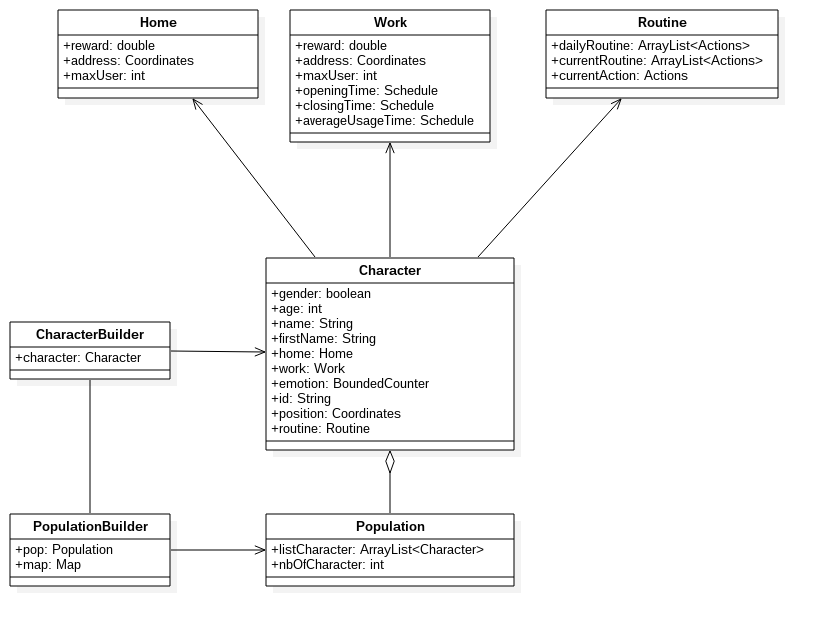
\includegraphics[width=400pt]{images/pop.png}
  \caption{Organisation de la partie population} \label{fig:population}
\end{figure}
 
 \paragraph{}
 La classe PopulationBuilder va construire une population gr�ce � la carte de jeu (pour assigner les r�sidences) et gr�ce au CharacterBuilder. 
 Ce dernier va faire la lecture dans les fichiers CSV gr�ce � la biblioth�que Apache-commons-csv et va faire les choix al�atoires pour initialiser les diff�rentes composantes de nos personnages.
 
 \subsection{Le moteur de jeu}
 
 \subsubsection{Gestion de l'�motion des personnages}
 
 \paragraph{}
 L'�motion repr�sente la barre de vie des personnages, elle varie de 0 � 100 en fonction du temps. 
 Si elle atteint 0, le personnage meurt. 
 L?�volution de cette jauge d?�motion est totalement dynamique, elle se fera automatiquement en fonction des actions faites par le personnage. 
 Certaines actions vont apporter un bonus sur la jauge d'�motion du personnage alors que d'autres vont apporter un malus. 
 Pour certaines actions le bonus est constant (par exemple dormir apportera toujours +30) mais pour d'autres le bonus/malus est variable en fonction du lieu dans lequel se fait l'action. 
 Par exemple travailler dans un atelier auto apportera un malus de -25 car la tache est difficile alors que travailler dans une boutique d?�lectronique apportera un malus de -15. 
 M�me fonctionnement pour les bonus des loisirs. 
 Ces valeurs sont initialiser lors que l'initialisation des b�timents, elles proviennent donc d'un fichiers CSV. 
 Enfin les rewards de sont pas toujours effectif au m�me moment. 
 Pour la plupart des actions, le personnage per�oit le reward en fin d'action. 
 Pour l'action de d�placement, dans un soucis de mieux repr�senter la r�alit�, le malus est retir� � chaque it�ration de temps. 
 C'est � dire que plus le chemin que le personnage a � faire est long, plus il perd de l'�motion.
 
 \begin{tabular} {|p{3.5cm}|p{5cm}|p{5cm}|}
\hline
Action & Reward & Effectivit� \\
\hline
Sleeping & +30 & En fin d'action \\
\hline
Chilling & +5 & En fin d'action \\
\hline
Schifting & -1 & A chaque it�ration de temps \\
\hline
Working & Malus variable [-25;-10] & En fin d'action \\
\hline
Entertain & Bonus variable [+5;+20] & En fin d'action \\
\hline
\end{tabular}

\subsubsection{Gestion de la routine}
\paragraph{}
La routine est un encha�nement d'actions que va ex�cuter le personnage. 
Le personnage peut ex�cuter 5 types d'actions diff�rentes regrouper en familles�: les d�placements et les occupations.  
Les actions d'occupation sont reli�es � un lieu alors que les actions de d�placement sont reli�es � un lieu de d�part, un lieu d'arriv� et un chemin entre les deux.


\begin{figure}[!h] 	
  \centering 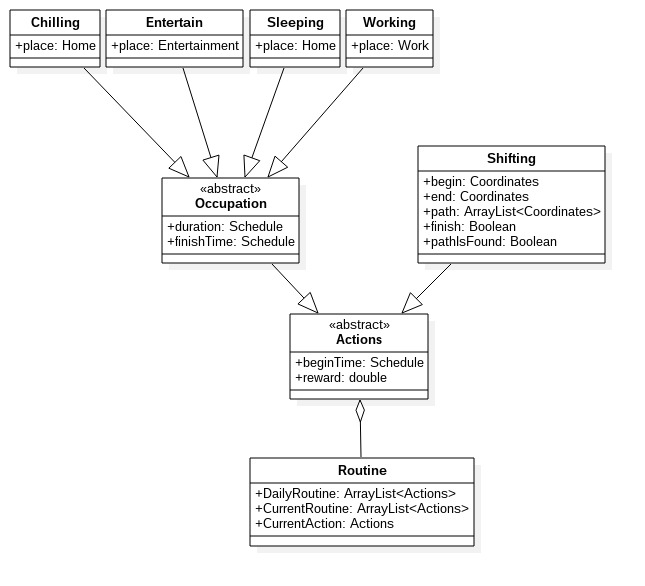
\includegraphics[width=400pt]{images/routine.jpg}
  \caption{Classe routine} \label{fig:characterClass}
\end{figure}

\paragraph{}
L'un des dilemme du projet est l?interaction entre les diff�rentes actions pour  que chaque personnage puisse avoir puisse suivre une suite d'actions ind�pendantes mais que l'utilisateur puisse ajouter des actions a faire sans perturber le bonne encha�nement des actions.

\paragraph{}
Nous avons d�cid� de d�composer ce probl�me en 3 partie�:
\begin{itemize}
 \item Une partie statique qui organise les grandes lignes des journ�es du personnage�: m�tro/boulot/dodo
 \item Une partie dynamique qui �volue au court de la journ�e et qui repr�sente la liste d'actions que le personnage a � faire
 \item Une partie utilisateur associ� � diff�rente options d'ajout/suppression d'actions 
\end{itemize}

\begin{figure}[!h] 	
  \centering 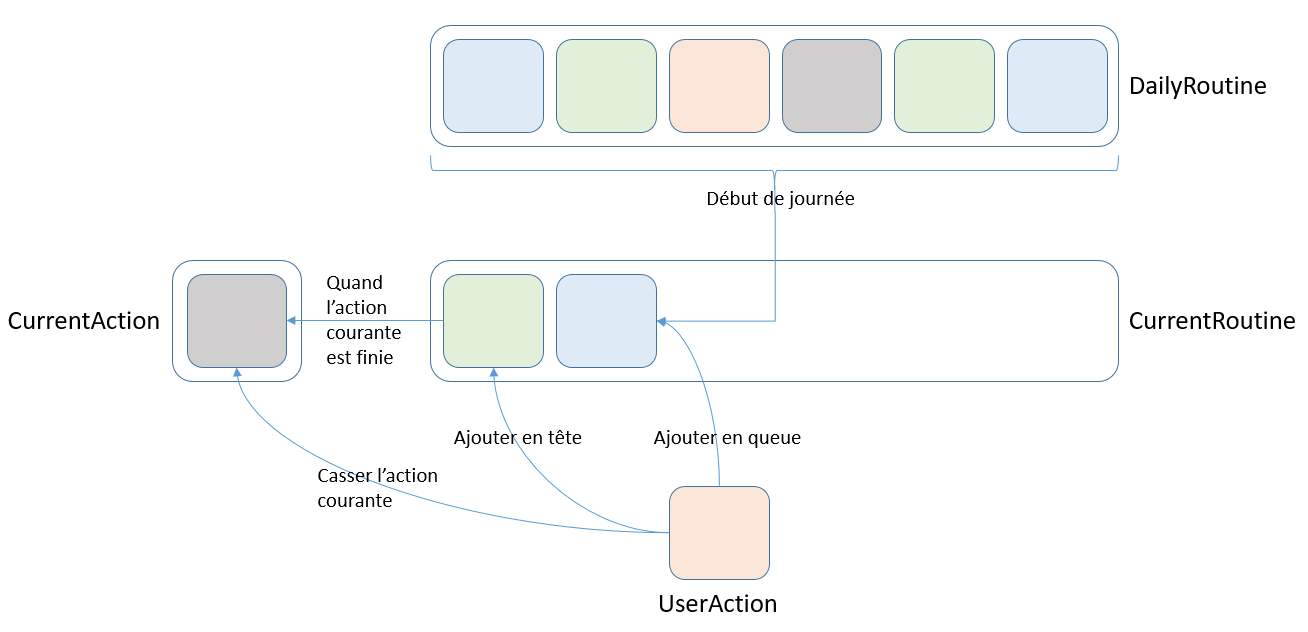
\includegraphics[width=400pt]{images/schemaRoutine.PNG}
  \caption{Fonctionnement de la routine} \label{fig:fonctionnementRoutine}
\end{figure}

\paragraph{}
La liste d'actions communes a chaque journ�es est stock� dans la liste DailyRoutine. 
A chaque d�but de journ�e, on ajoute toutes les actions de cette liste a la de la journ�e courante, CurentRoutine. 
La currentRoutine � les m�me propri�t�s qu'une files mais avec plus de possibilit� d'ajout d'actions. 
On d�file currentRoutine et on ajoute cette action � l'action courante, currentAction. 
Cette action est ex�cut� par le personnage et lorsqu'elle est finie, on d�file � nouveau la currentRoutine. 
Enfin l'utilisateur peut soit ajouter un action en t�te ou en queue dans la currentRoutine ou il peut casser l'action courante du personnage mais cela engendra un malus d?�motion.

\subsubsection{Calcul d'itin�raire}

\subsection{L'interface homme/machine}

\paragraph{}
L'interface graphique est compos� de plusieurs �l�ments�:
\begin{itemize}
 \item L'horloge du jeu, permettant de savoir quelle est la date et l'heure dans notre ville fictive
 \item La map, ou nous pouvons voir les infrastructures, et les personnages se d�placer
 \item La liste des personnages accompagn� de l'�tat de leur barre d'�motion
\end{itemize}

\paragraph{}
Chacun de ces �l�ments sont s�par� dans diff�rentes classes qui h�ritent de la classe JPanel , ce qui permet un assemblage facile de l'interface graphique, et une permutation plus facile entre diff�rentes versions d'un m�me �l�ments.

\paragraph{}
L'interface graphique est r�alis� gr�ce � Java Swing/AWT/Java 2D .

\paragraph{}
Nous pouvons voir dans le diagramme ci dessus que l'ensemble des �l�ments graphiques sont rassembl� dans une seule classe principale, qui � pour but de les assembler correctement.

\paragraph{}
La Map et la liste des personnages sont cliquables et affiche des informations en fonction de la position du curseur au moment du clique. 
Cela peut permettre d'ouvrir un autre Panel, une autre fen�tre ou autre, contenant les informations souhait�es, en fonction des situations (Pour plus de d�tail, se reporter au manuel d'utilisation). 
Ces fonctionnalit�s ont �t� impl�ment� gr�ce � des MouseListener, qui nous permettent de r�cup�rer des informations sur le curseur ou l'�tat de la souris/trackpad lors d'�v�nements pr�d�fini, lors d'un clic de souris par exemple.


%R�f�rences bibliographiques du document
\bibliographystyle{plain}
\bibliography{bibliographies}
\nocite{*}

\end{document}
